\section{Empirical Studies of the Effectiveness of SOMA}\label{sec:exp}

We evaluate SOMA through five questions. \textbf{RQ1}: Can a small surrogate preserve the original model's responses? \textbf{RQ2}: Does higher response similarity also improve task-grounded quality? \textbf{RQ3}: When does SOMA provide net efficiency gains after warm-start and adaptation overhead? \textbf{RQ4}: Which components of SOMA are most important? \textbf{RQ5}: When is session-local serving reliable, and when should SOMA fall back to the large model?

\textbf{Datasets.} We evaluate SOMA on six multi-turn benchmarks: ShareGPT~\citep{chen2024sharegpt4v}, ReMeDi~\citep{yan2022remedi}, Craigslist~\citep{he2018decoupling}, Multi-Char~\citep{agentlans_multi-character_dialogue_2024}, MATH~\citep{hendrycks2021measuring}, and MT-Bench~\citep{zheng2023judging}. Dataset details and the context-dependence filtering are in Appendix~\ref{sec:app_dataset}.

\textbf{Models and baselines.} We test two model families: LLaMA, using LLaMA-3.1-70B as \(F\) and LLaMA-2-7B as \(G\), and Qwen, using Qwen-3-8B as \(F\) and Qwen-3-0.6B as \(G\). We compare with Original, Surrogate, History-Prefix, History-FT, LLMLingua-2~\citep{pan2024llmlingua}, and RouteLLM~\citep{ong2024routellmlearningroutellms}; Appendix~\ref{sec:app_baseline} details each baseline.

\textbf{Metrics.} We mainly measure teacher-fidelity similarity, i.e., how closely each method preserves the original model's response, using three LLM judges: GPT-OSS~\citep{openai2025gptoss120bgptoss20bmodel}, DeepSeek-V3, and Gemma-2-27B. To complement similarity with task-grounded quality, we report EM accuracy on MATH. Efficiency is measured by token usage, throughput, and end-to-end \rev{wall-clock} latency, \rev{which for SOMA includes soft-prompt mining, LoRA adaptation, and gating. All models run on vLLM~0.10.2 with automatic prefix caching, so every baseline reuses the KV cache across turns.}

\textbf{Implementation.} We set the warm-start window, acceptance batch, candidate count, and switch threshold from Section~\ref{sec:theory}; after switching, SOMA performs no further LoRA updates and keeps only the drift check. Appendix~\ref{sec:app_implementation} lists all hyperparameters.

\subsection{Experimental Results}
\label{sec:exp_res}

\paragraph{\textbf{RQ1: Response similarity to the original model.}}

\begin{table}[!t]
\centering
\caption{Response similarity to the original model on the LLaMA family. Higher is better. \rev{SOMA stays closest to the original model on all six datasets. It raises the average from 75.1 for the unadapted surrogate to 93.1, 0.9 points above the strongest baseline, RouteLLM.}}
\label{tab:llama-pct}
\resizebox{0.96\textwidth}{!}{
\begin{tabular}{lccccccc}
\toprule
 & \textbf{ShareGPT} & \textbf{ReMeDi} & \textbf{Craigslist} & \textbf{Multi-Char} & \textbf{MATH} & \textbf{MT-Bench} & \textbf{Avg.} \\
\midrule
Surrogate      & 79.2 $\pm$ 2.18 & 82.7 $\pm$ 1.95 & 74.3 $\pm$ 2.36 & 70.8 $\pm$ 1.73 & 66.2 $\pm$ 2.91 & 77.5 $\pm$ 2.04 & 75.1 $\pm$ 5.98 \\
History-Prefix & 86.1 $\pm$ 1.67 & 87.9 $\pm$ 1.55 & 82.4 $\pm$ 1.72 & 84.7 $\pm$ 1.69 & 80.3 $\pm$ 3.83 & 87.2 $\pm$ 1.58 & 84.8 $\pm$ 2.94 \\
History-FT     & 93.4 $\pm$ 2.12 & 91.8 $\pm$ 2.09 & 90.3 $\pm$ 1.23 & 89.1 $\pm$ 2.23 & 87.6 $\pm$ 2.26 & 92.4 $\pm$ 1.14 & 90.8 $\pm$ 2.18 \\
LLMLingua-2    & 84.6 $\pm$ 1.72 & 86.4 $\pm$ 1.63 & 80.8 $\pm$ 1.91 & 82.9 $\pm$ 1.58 & 78.1 $\pm$ 2.77 & 85.3 $\pm$ 1.66 & 83.0 $\pm$ \rev{3.11} \\
RouteLLM       & 95.3 $\pm$ 1.44 & 92.5 $\pm$ 1.07 & 91.0 $\pm$ 1.86 & 91.4 $\pm$ 1.23 & 89.6 $\pm$ 1.95 & 93.2 $\pm$ 1.12 & 92.2 $\pm$ \rev{1.98} \\
\midrule
\textbf{SOMA}  & \textbf{96.4 $\pm$ 1.91} & \textbf{93.2 $\pm$ 0.98} & \textbf{91.9 $\pm$ 2.49} & \textbf{92.3 $\pm$ 1.05} & \textbf{90.7 $\pm$ 1.12} & \textbf{94.1 $\pm$ 0.91} & \textbf{93.1 $\pm$ 1.99} \\
\bottomrule
\end{tabular}}
\vspace{-3mm}
\end{table}

\begin{table}[!t]
\centering
\caption{Response similarity to the original model on the Qwen family. Higher is better. \rev{SOMA again leads on all six datasets. Similarities are lower than for LLaMA, probably because the size gap is wider, and SOMA's average gain over the unadapted surrogate grows to 27.1 points.}}
\label{tab:qwen-pct}
\resizebox{0.96\textwidth}{!}{
\begin{tabular}{lccccccc}
\toprule
 & \textbf{ShareGPT} & \textbf{ReMeDi} & \textbf{Craigslist} & \textbf{Multi-Char} & \textbf{MATH} & \textbf{MT-Bench} & \textbf{Avg.} \\
\midrule
Surrogate       & 50.9 $\pm$ 1.21 & 63.5 $\pm$ 2.87 & 48.2 $\pm$ 3.40 & 44.7 $\pm$ 3.54 & 42.6 $\pm$ 1.70 & 40.4 $\pm$ 0.81 & 48.4 $\pm$ 8.31 \\
History-Prefix  & 70.5 $\pm$ 1.15 & 75.7 $\pm$ 2.01 & 63.0 $\pm$ 2.23 & 65.5 $\pm$ 0.91 & 51.3 $\pm$ 2.45 & 53.6 $\pm$ 2.32 & 63.3 $\pm$ 9.47 \\
History-FT      & 76.4 $\pm$ 1.68 & 79.2 $\pm$ 2.61 & 74.5 $\pm$ 3.56 & 63.2 $\pm$ 1.74 & 65.9 $\pm$ 1.70 & 62.7 $\pm$ 0.72 & 70.3 $\pm$ 7.23 \\
LLMLingua-2     & 68.9 $\pm$ 1.32 & 74.1 $\pm$ 2.14 & 61.2 $\pm$ 2.67 & 63.4 $\pm$ 1.18 & 49.8 $\pm$ 2.03 & 51.7 $\pm$ 1.45 & 61.5 $\pm$ \rev{9.49} \\
RouteLLM        & 79.6 $\pm$ 1.04 & 81.9 $\pm$ 1.36 & 75.1 $\pm$ 2.91 & 72.8 $\pm$ 1.62 & 67.3 $\pm$ 1.21 & 68.0 $\pm$ 0.96 & 74.1 $\pm$ \rev{5.95} \\
\midrule
\textbf{SOMA}   & \textbf{81.0 $\pm$ 0.93} & \textbf{83.2 $\pm$ 1.21} & \textbf{76.4 $\pm$ 3.85} & \textbf{74.2 $\pm$ 2.53} & \textbf{68.7 $\pm$ 1.28} & \textbf{69.2 $\pm$ 1.08} & \textbf{75.5 $\pm$ 5.97} \\
\bottomrule
\end{tabular}}
\vspace{-3mm}
\end{table}

\begin{table}[!t]
\centering
\caption{MATH exact-match accuracy. \rev{SOMA stays below the original model but recovers 77--78\% of the gap between the surrogate and the original model and outperforms every other baseline.}}
\label{tab:math-em}
\resizebox{\textwidth}{!}{
\begin{tabular}{lcccccc}
\toprule
\textbf{Family} & \textbf{Orig.} & \textbf{Surr.} & \textbf{Hist.-P} & \textbf{Hist.-FT} & \textbf{Route} & \textbf{SOMA} \\
\midrule
LLaMA & 48.34 $\pm$ 0.32 & 19.20 $\pm$ 0.78 & 25.03 $\pm$ 0.94 & 31.46 $\pm$ 0.87 & 33.88 $\pm$ 0.79 & \textbf{41.62 $\pm$ 0.66} \\
Qwen  & 36.48 $\pm$ 0.41 & 11.73 $\pm$ 0.64 & 16.21 $\pm$ 0.79 & 22.57 $\pm$ 0.83 & 25.08 $\pm$ 0.71 & \textbf{31.14 $\pm$ 0.74} \\
\bottomrule
\end{tabular}}
\vspace{-3mm}
\end{table}

After the warm-start stage, the surrogate should preserve the original model's behavior within the current dialogue state. Table~\ref{tab:llama-pct} reports response similarity on the LLaMA family. SOMA achieves the highest average similarity across all six datasets. The gap over Surrogate shows the behavior loss caused by directly replacing the large model with a smaller model. The gap over History-FT shows that local adaptation helps, \rev{and seems to help more when the warm-start turns are weighted by their anchoring scores.} The largest gains appear on MATH and Multi-Char, where later turns depend on accumulated reasoning states, constraints, and roles. \rev{Table~\ref{tab:qwen-pct} repeats the evaluation on the Qwen family. Absolute similarities are lower, likely because the capacity gap between Qwen-3-8B and Qwen-3-0.6B is wider and local imitation becomes harder. SOMA is still the best method on every dataset.}

\paragraph{\textbf{RQ2: Task-grounded quality.}}
Response similarity is the primary metric for replacing the original model, but similarity alone does not guarantee task quality. We therefore evaluate MATH using exact-match accuracy. Table~\ref{tab:math-em} shows that SOMA remains below the original large model, as expected, but substantially narrows the gap between the surrogate and the original model. SOMA also outperforms History-Prefix, History-FT, and RouteLLM in both model families. Thus SOMA's gains are not only surface-level matching: local adaptation also preserves more of the original model's reasoning.

\paragraph{\textbf{RQ3: End-to-end efficiency.}}

\begin{figure}[!t]
\centering
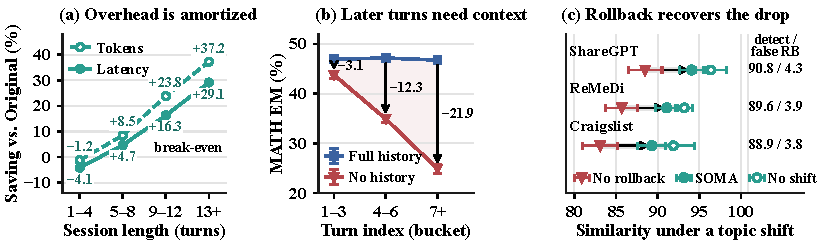
\includegraphics[width=\textwidth]{figure/operating.pdf}
\vspace{-5mm}
\caption{Operating range and reliability. (a) End-to-end saving of SOMA over Original on ShareGPT after all warm-start and adaptation overhead, by session length. (b) MATH exact match with and without the dialogue history: later turns remain context-dependent. (c) Response similarity under an abrupt topic shift without rollback, with SOMA's drift-aware rollback, and without a shift; the right column lists SOMA's shift-detection and false-rollback (RB) rates in \%.}
\label{fig:operating}
\vspace{-3mm}
\end{figure}

\begin{figure}[!t]
  \centering
  \begin{subfigure}[t]{0.49\textwidth}
    \centering
    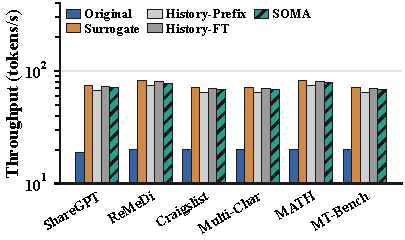
\includegraphics[width=\linewidth]{figure/llama_through.pdf}
    \caption{LLaMA family.}
  \end{subfigure}\hfill
  \begin{subfigure}[t]{0.49\textwidth}
    \centering
    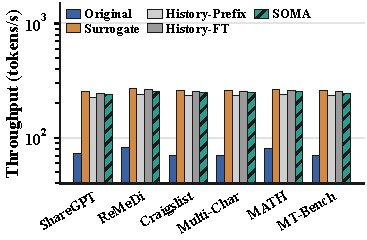
\includegraphics[width=\linewidth]{figure/qwen_through.pdf}
    \caption{Qwen family.}
  \end{subfigure}
  \vspace{-2mm}
  \caption{Throughput across six datasets. SOMA keeps the serving path close to the surrogate while maintaining higher similarity to the original model.}
  \label{fig:app_throughput}
\vspace{-3mm}
\end{figure}

SOMA reduces post-switch cost by serving the adapted surrogate with compressed context, but it also introduces one-time costs from soft-prompt probing and LoRA adaptation. Thus, the key question is whether the total session cost decreases after this overhead is included. SOMA reduces average token usage by avoiding repeated full-history serving after switching (Appendix~\ref{sec:app_eff}). Figure~\ref{fig:operating}(a) further shows the amortized operating range: \rev{SOMA is slightly unfavorable for sessions of 1--4 turns ($-4.1\%$ latency) and roughly breaks even at 5--8 turns ($+4.7\%$). From 9 turns on, it saves $16.3\%$ to $29.1\%$ latency and $23.8\%$ to $37.2\%$ tokens.} This matches SOMA's intended use case as an amortized serving strategy for conversations where enough later turns remain local to the warm-start state. \rev{Figure~\ref{fig:app_throughput} reports throughput on all six datasets for both families. SOMA runs at 95--97\% of the throughput of Surrogate and History-FT, about 5.6\% faster than History-Prefix and 3.1--3.9$\times$ faster than Original. Appendix~\ref{sec:app_eff} lists the per-dataset token costs.}

\paragraph{\textbf{RQ4: Component contributions.}}

We first ablate SOMA on the LLaMA family to identify which components drive the gains. Figure~\ref{fig:llama_ablation} shows that full SOMA performs best across all datasets. Removing the anti-degeneration loss consistently reduces performance, showing that entropy regularization keeps prompt mining stable and prevents collapsed, low-diversity soft prompts. Removing both the expectation-weighted term and the anti-degeneration loss leads to a larger drop, especially on harder datasets. \rev{This result suggests that the anchoring scores are most informative when the probe is both stable and semantic.} \rev{Figure~\ref{fig:qwen_ablation} repeats the ablation on the Qwen family and finds the same ordering, so the conclusion does not appear to hinge on the backbone. Figure~\ref{fig:mt_radar} breaks MT-Bench-101 down by ability for the LLaMA family. Relative to the surrogate, SOMA gains most on reasoning, reflection, and questioning, and it also improves understanding, interference handling, memory, and rephrasing to a smaller degree.}

% \begin{figure}[t]
%   \centering
%   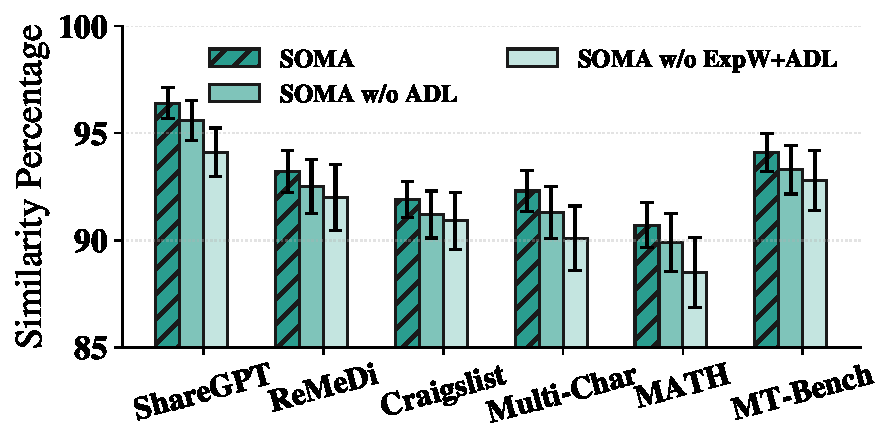
\includegraphics[width=0.70\textwidth]{figure/ablation_llama.pdf}
%   \caption{Ablation study on the LLaMA family. Full SOMA performs best, confirming the importance of anti-degeneration regularization and expectation-weighted divergence in soft-prompt mining.}
%   \label{fig:ablation-llama}
% \end{figure}

\paragraph{\textbf{RQ5: Reliability and fallback.}}

\begin{figure}[!t]
  \centering
  \begin{subfigure}[t]{0.344\textwidth}
    \centering
    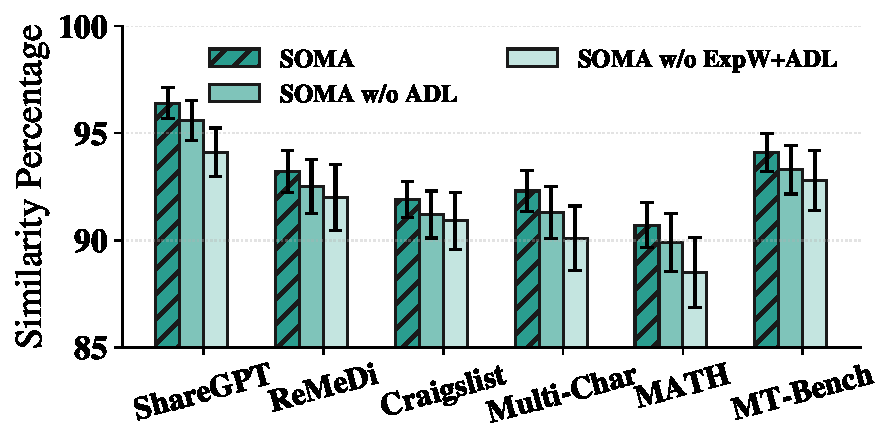
\includegraphics[width=\linewidth]{figure/ablation_llama.pdf}
    \caption{LLaMA ablation.}
    \label{fig:llama_ablation}
  \end{subfigure}\hfill
  \begin{subfigure}[t]{0.344\textwidth}
    \centering
    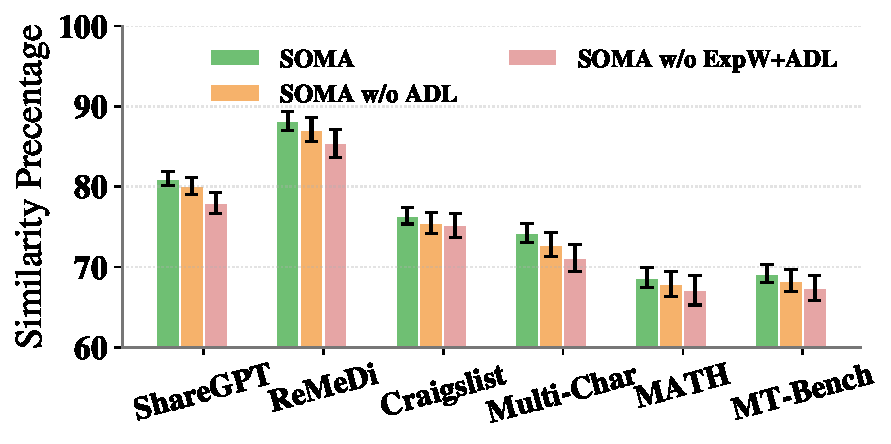
\includegraphics[width=\linewidth]{figure/ablation_qwen.pdf}
    \caption{Qwen ablation.}
    \label{fig:qwen_ablation}
  \end{subfigure}\hfill
  \begin{subfigure}[t]{0.281\textwidth}
    \centering
    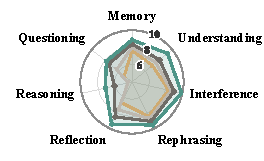
\includegraphics[width=\linewidth]{figure/mt_radar.pdf}
    \caption{Ability profile.}
    \label{fig:mt_radar}
  \end{subfigure}
  \vspace{-2mm}
  \caption{Component and capability analysis. Anti-degeneration regularization and expectation-weighted divergence both improve mining on LLaMA (a) and Qwen (b). (c) MT-Bench-101 ability profile of \textbf{Surrogate}~\textcolor{radarsur}{$\blacktriangle$}, \textbf{History-Prefix}~\textcolor{radarhp}{$\blacktriangledown$}, \textbf{History-FT}~\textcolor{radarft}{$\blacklozenge$}, and \textbf{SOMA}~\textcolor{radarsoma}{$\bullet$}.}
  \label{fig:token_ablation}
\vspace{-3mm}
\end{figure}

\begin{figure}[!t]
  \centering
  \begin{subfigure}[t]{0.525\textwidth}
    \centering
    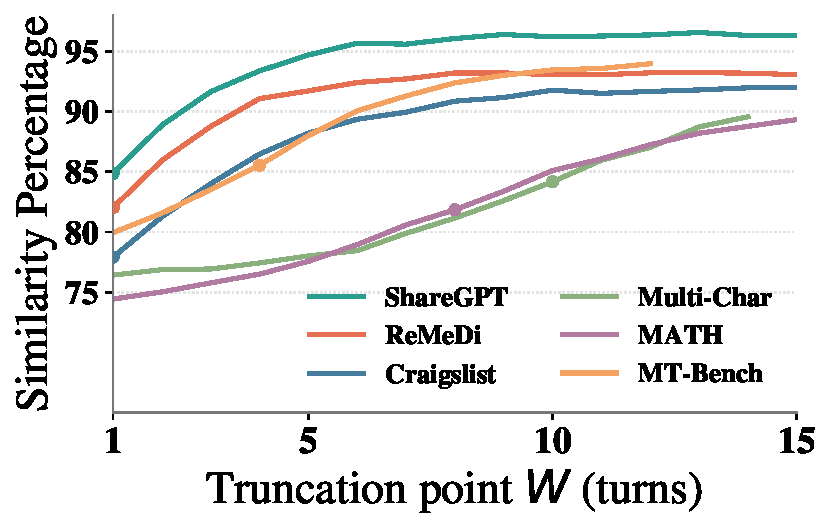
\includegraphics[width=\linewidth]{figure/truncation_trend.pdf}
    \caption{Similarity under different switch points.}
  \end{subfigure}\hfill
  \begin{subfigure}[t]{0.445\textwidth}
    \centering
    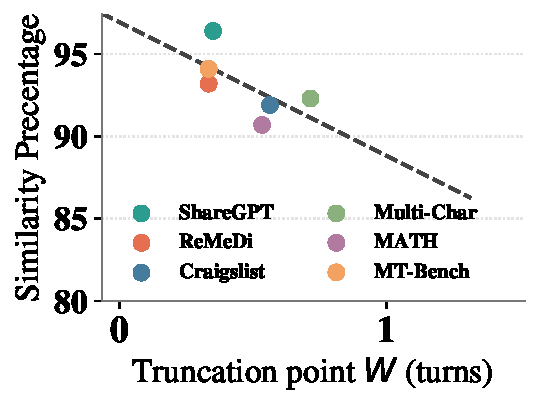
\includegraphics[width=\linewidth]{figure/truncation_vs_similarity.pdf}
    \caption{\rev{Relative switch point} vs.\ final similarity.}
  \end{subfigure}
  \vspace{-2mm}
  \caption{Warm-start and switching behavior. Easier local-dialogue settings switch earlier, while reasoning-heavy or multi-party settings need longer warm starts and achieve lower final similarity.}
  \label{fig:app_switching}
\vspace{-3mm}
\end{figure}

We next test when SOMA's locality assumption holds and how rollback helps when it fails. Figure~\ref{fig:operating}(b) shows that full-history MATH performance stays stable across turn buckets, while no-history performance drops sharply in later turns\rev{, from a 3.1-point EM loss on turns 1--3 to a 21.9-point loss on turns 7 and later}. This means later turns are not simply easier; they remain strongly dependent on the earlier dialogue context. Figure~\ref{fig:operating}(c) then evaluates abrupt topic shifts. Without rollback, similarity drops substantially. With SOMA's drift-aware rollback, \rev{similarity returns to within 2.1--2.6 points of the clean setting (e.g., $88.5\to94.1$ vs.\ $96.4$ on ShareGPT), with 88.9--90.8\% of shifts detected and 3.8--4.3\% false rollbacks.} These results show that SOMA should be viewed as a local serving strategy with automatic fallback. \rev{Figure~\ref{fig:app_switching} shows the warm-start side. Goal-anchored dialogues (ShareGPT, ReMeDi, Craigslist) reach high similarity after a few turns, while reasoning-heavy or multi-party ones (MATH, Multi-Char) need longer warm starts and level off lower. The best switch point thus seems data-dependent, and the gate picks it per session.}

